\documentclass[11pt, a4paper, USenglish]{article} % change ``USenglish'' to ``norsk'' if applicable.

% Search http://ctan.org or type texdoc <package name> in a terminal to access LaTeX package documentation.
\usepackage{float}
\usepackage[parfill]{parskip}
\usepackage{babel} % babel and csquotes are packages for multilingual (e.g. Norwegian) support.
\usepackage[T1]{fontenc} % See http://tex.stackexchange.com/questions/664/why-should-i-use-usepackaget1fontenc
\usepackage[utf8]{inputenc} % See http://tex.stackexchange.com/questions/44694/fontenc-vs-inputenc
\usepackage{csquotes} % Needs to be loaded after inputenc.
\usepackage{amsmath} % See: http://tex.stackexchange.com/questions/32100/what-does-each-ams-package-do
\usepackage{amssymb} % See above.
\usepackage[squaren]{SIunits} % Provides SI units like \meter. The squaren option is due to a conflict with amssymb.
\usepackage{graphicx} % Provides the \includegraphics command.
\usepackage{booktabs} % Better tables. Provides \toprule, \midrule, \bottomrule.
\usepackage{listings} % Provides source code listings.
\usepackage{todonotes} % Provides several handy TODO commands.
\usepackage[
  backend=bibtex,
  style=numeric,
  isbn=false,
  doi=false]{biblatex} % http://tex.stackexchange.com/questions/25701/bibtex-vs-biber-and-biblatex-vs-natbib
\usepackage{hyperref} % Provides clickable links. Always load last, but before cleveref.
\usepackage{cleveref} % Provides the \Cref command, for cross-referencing of equations, sections, figures and tables. Always load last.
\usepackage{epstopdf}
\usepackage{caption}
\usepackage{varwidth}
\DeclareCaptionFormat{myformat}{%
  % #1: label (e.g. "Table 1")
  % #2: separator (e.g. ": ")
  % #3: caption text
  \begin{varwidth}{\linewidth}%
    \centering
    #1#2#3%
  \end{varwidth}%
}
\usepackage{lipsum}
\usepackage{titlesec}
\usepackage{caption,setspace}
\captionsetup{font={stretch=1.0}}

\addbibresource{bibliography.bib} % Makes the bibliography file available to biblatex.

% ``listings'' package settings
\definecolor{dkgreen}{rgb}{0,0.6,0}
\definecolor{gray}{rgb}{0.5,0.5,0.5}
\definecolor{pink}{rgb}{0.63, 0.13, 0.94}
\lstset{language=Matlab, 
	keywords={break, case, catch, continue,else,elseif,end,for,function,
		global,if,otherwise,persistent,return,switch,try,while},
	basicstyle=\ttfamily,
	keywordstyle=\color{blue},
	commentstyle=\color{dkgreen},
	stringstyle=\color{pink},
	numbers=left,
	numberstyle=\tiny\color{gray},
	stepnumber=1,
	numbersep=10pt,
	backgroundcolor=\color{white},
	tabsize=4,
	showspaces=false,
        showstringspaces=false}
 % The preamble specifies all included packages and related parameters.
% \input simply inserts the contents of the file, while \include forces a \newpage.
% See \input vs. \include: http://tex.stackexchange.com/questions/246/when-should-i-use-input-vs-include

\begin{document}

% Titlepage
\title{TTK4135 Optimization and Control\linebreak Helicopter Lab}
\author{Group 66\\Student 999239\\Student 999526\\Student 481882}
\date{April 28, 2017}
\begin{titlepage}
    \maketitle
    \begin{figure}
    \centering
    
\includegraphics[width=0.5\textwidth]{figures/itk_ntnu}\\
    Department of Engineering Cybernetics
    \end{figure}
    \thispagestyle{empty}
\end{titlepage}

% Abstract
\newpage
\pagenumbering{roman}
\setlength{\parskip}{1em}
%\renewcommand{\baselinestretch}{2.0}
\begin{abstract} 
%\addcontentsline{toc}{section}{Abstract} % add this if you want the abstract in the table of contents.
\noindent
This lab is an introduction to how optimization and control theory can be implemented in physical systems. The problems are solved using the computer software MATLAB and Simulink, and are tested in a safe environment in which a fixed electrical flying object is manipulated to fly on a  calculated trajectory. A given set of states are controlled with and without feedback and constraints.\\
\\
We want to thank the student assistants for giving us guidance through this exercise and leading us to a feasible result. 
\end{abstract}

%\thispagestyle{empty} % Avoid page numbering on the abstract page.

% TOC
\newpage
\tableofcontents
%\thispagestyle{empty} % Avoid page numbering on the table of contents.

% Main content
\newpage
\pagenumbering{arabic}
\section{Introduction}\label{sec:intro}
The very first day of this lab exercise was spent repeating/getting to know the developing- and control environment, Simulink and QuaRC, before moving on to making an optimal control system to calculate the optimal trajectory of a fixed helicopter. In this report the reader is first shown the physical model that forms the basis of the control problem. Section \ref{sec:10.2} explains how an optimal input sequence is calculated and implemented without feedback, to move the helicopter from 0 to 180 degrees. In this case only pitch and travel is controlled. Feedback is then implemented in Section \ref{sec:10.3}, and in Section \ref{sec:10.4} an extra dimension is introduced - elevation. Each section is ended off with a section of results and discussion. The main goal of the report is to give a glance into how optimal control can be implemented to ensure optimal control of physical systems. In practice, this could mean saving fuel, wear or getting just the right set points in a chemical reactor - which again means helping the environment and lowering costs. 












\section{Problem Description}\label{sec:prob_descr}

The system consists of an arm suspended on a base which can rotate freely around a vertical axis. On one end of the arm is the helicopter, consisting of two DC motors with rotor blades which are partially encased for safety. On the other end there is a counter weight which is adjusted so that the weight lifted from the motors are approximately 40g. A Quanser Q4 i used as a control board.


\begin{figure}[H]
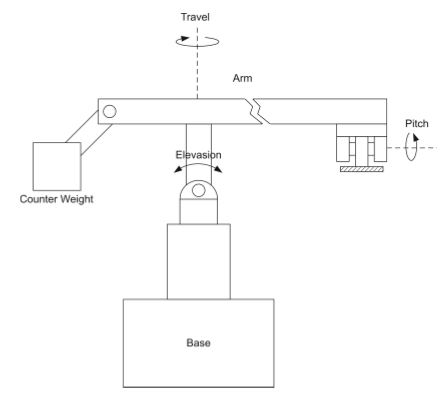
\includegraphics[width=1\linewidth, height=10cm]{figures/Helikopter.JPG}
\caption{The helikopter system}\label{fig:figur9}
\end{figure}

\newpage
\subsection{Model Derivation}\label{sec:mod_der}
A mathematical model for the system is derived from first principles. 

For elevation we have:

\begin{subequations}
\begin{equation}\label{eq:model_elevation1}
J_{e} \ddot{e} = l_{a} K_{f} V_{s} - T_{g}
\end{equation}

\begin{equation}\label{eq:model_elevation2}
\ddot{e} = K_{3} V_{s} - \frac{T_{g}}{J_{e}}\,\quad K_{3} = \frac{l_{a}K_{f}}{J_{e}}\
\end{equation}
\end{subequations}

The pitch is controlled by a PD controller and is modelled in the following way:

\begin{subequations}
\begin{equation}\label{eq:model_pitch1}
J_{p} \ddot{p} = l_{h} K_{f} V_{d}
\end{equation}

\begin{equation}\label{eq:model_pitch2}
\ddot{p} = K_{1} V_{d},\quad K_{1} = \frac{l_{h}K_{f}}{J_{p}}\
\end{equation}
\end{subequations}

The horizontal component of the force from the helicopter gives us the acceleration around the travel axis:

\begin{subequations}
\begin{equation}\label{eq:model_travel1}
\ddot{p} = -K_{p} l_{a} sin(p)
\end{equation}

\begin{equation}\label{eq:model_travel2}
\dot{r} = -K_{2}p,\quad K_{2} = \frac{l_{a}K_{p}}{J_{t}}\
\end{equation}
\end{subequations}

\newpage
\subsection{Assumptions, Limitations and the Final Model}
All controllers are assumed properly tuned in this project, and also that the motors output a force which is proportional to the voltage applied to them. The elevation is controlled by a PID controller and we assume that the constant term \(\frac{T_{g}}{J_{e}}\) is cancelled out by the integral term. We also assume that the pitch angle is small, such that the force to keep the helicopter flying is approximately \(K_{p}\) and \(\sin(p)=p\). This is not the case and will be a source of error. Taking these into account we end up with the final model:

\begin{subequations}\label{eq:model_al}
	\begin{align}
		\ddot{e} + K_{3} K_{ed} \dot{e} + K_{3} K_{ep} e &= K_{3} K_{ep} e_{c} \label{eq:model_se_al_elev} \\
		\ddot{p} + K_{1} K_{pd} \dot{p} + K_{1} K_{pp} p &= K_{1} K_{pp} p_{c} \label{eq:model_se_al_pitch} \\
		\dot{\lambda} &= r \label{eq:model_se_al_lambda} \\
		\dot{r} &= -K_{2} p \label{eq:model_se_al_r} 
	\end{align}
\end{subequations}

Parameters and variables are given in table 1 and 2.


\newpage
\begin{table}[tbp]
	\centering
	\caption{Parameters and values}
	\begin{tabular}{l1ll}
		\toprule
		Symbol & Parameter & Value & Unit \\
		\midrule
		$l_a$ & Distance from elevation axis to helicopter body & $0.63$ & \meter\\
		$l_h$ & Distance from pitch axis to motor & $0.18$ & \meter\\
		$K_f$ & Force constant motor & $0.25$ & \newton\per\volt\\
		$J_e$ & Moment of inertia for elevation & $0.83$ & \kilogram\usk\meter\squared\\
		$J_t$ & Moment of inertia for travel & $0.83$ & \kilogram\usk\meter\squared\\
		$J_p$ & Moment of inertia for pitch & $0.034$ & \kilogram\usk\meter\squared\\
		$m_h$ & Mass of helicopter & $1.05$ & \kilogram\\
		$m_w$ & Balance weight & $1.87$ & \kilogram\\
		$m_g$ & Effective mass of the helicopter & $0.05$ & \kilogram\\
		$K_p$ & Force to lift the helicopter from the ground & $0.49$ & \newton\\
		\bottomrule
	\end{tabular}
\label{tab:parameters}
\end{table}

\newpage
\begin{table}[tbv]
	\centering
	\caption{Variables}
	\begin{tabular}{l1ll}
		\toprule
		Symbol & Variable \\
		\midrule
		$p$ & Pitch \\
		$p_{c}$ & Setpoint for pitch\\
		$\lambda$ & Travel\\
		$r$ & Speed of travel\\
		$r_{c}$ & Setpoint for speed of travel\\
		$e$ & Elevation\\
		$e_{c}$ & Setpoint for elevation \\
		$V_{f}$ & Voltage, motor in front\\
		$V_{b}$ & Voltage, motor in back\\
		$V_{d}$ & Voltage difference, \(V_{f}-V_{b}\)\\
		$V_{s}$ & Voltage sum, \(V_{f}+V_{b}\)\\
		$K_{pp},K_{pd},K_{ed},K_{ei},K_{ed}$ & Controller gains\\
		$T_{g}$ & Moment needed to keep the helicopter flying\\
		\bottomrule
	\end{tabular}
\label{tab:parameters}
\end{table}

\section[Optimal Control of Pitch/Travel without Feedback]{\setstretch{0.5}Optimal Control of Pitch/Travel \\ without Feedback}\label{sec:10.2}

In this section an optimal trajectory $x^*$ and a corresponding optimal input sequence $u^*$ is calculated. The calculated trajectory is used to bring the helicopter from its initial state to a desired final state. Elevation and feedback of the measured state are disregarded in this section.

\subsection{Continuous time state space form}
The model of the system can be written on continuous state space form 

\begin{equation}
\dot x = {A_c}x + {B_c}u
\end{equation}
\label{eq:statespace}

where $x=[\lambda\quad r\quad p\quad \dot p]^\top$ and $u=p_c$. The system matrices $A_c$ and $B_c$ are given by

\begin{subequations}
\begin{equation}
{A_c} = \left[ {\begin{array}{*{20}{c}}
0&1&0&0\\
0&0&{ - {K_2}}&0\\
0&0&0&1\\
0&0&{ - {K_1}{K_{pp}}}&{ - {K_1}{K_{pd}}}
\end{array}} \right]
\end{equation}\\
\begin{equation}
{B_c} = \left[ {\begin{array}{*{20}{c}}
0\\
0\\
0\\
{{K_1}{K_{pp}}}
\end{array}} \right]
\end{equation}
\end{subequations}\\

The model includes the basic control layer and the physical layer. The basic control layer consist of a PD controller for elevation control and a PID controller for pitch control, while the physical layer consist of the states connected to the helicopter. In regard to Figure \ref{fig:controlhierch}, which describes the system, the model is the two lower layers. The optimization layer is the layer we will focus on in this report. The optimal input sequence $u^*$ calculated will be implemented as setpoints for the inner controllers in the basic control layer.

\begin{figure}[H]
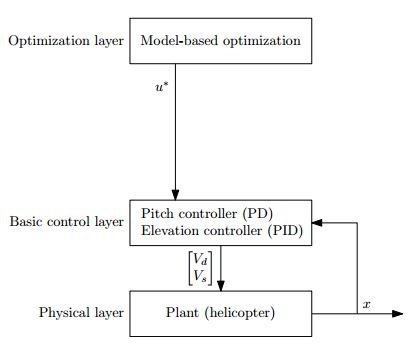
\includegraphics{figures/openLoopFlowChart}
\centering
\caption{Illustration of the layers in the control hierarchy}\label{fig:controlhierch}
\end{figure}

\subsection{Discrete time state space form}
The model is discretized by using the forward Euler method, given by
\begin{subequations}
\begin{equation}
{x_{k + 1}} = {x_k} + \Delta t({A_c}{x_k} + {B_c}{u_k})
\end{equation}
\begin{equation}
{x_{k + 1}} = (I + \Delta t{A_c}){x_k} + (\Delta t{B_c}){u_k}
\end{equation}
\label{eq:forwardeuler}
\end{subequations}

Thus, the model can be written on discrete time state space form
\begin{equation}
{x_{k + 1}} = A{x_k} + B{u_k}
\end{equation}

where 

\begin{subequations}
\begin{equation}
A = I + \Delta t{A_c} = \left[ {\begin{array}{*{20}{c}}
1&\Delta t&0&0\\
0&1&{ - \Delta t{K_2}}&0\\
0&0&1&\Delta t\\
0&0&{ - \Delta t{K_1}{K_{pp}}}&{1 - \Delta t{K_1}{K_{pd}}}
\end{array}} \right]
\end{equation}\\

\begin{equation}
B = \Delta t{B_c} = \left[ {\begin{array}{*{20}{c}}
0\\
0\\
0\\
{\Delta t{K_1}{K_{pp}}}
\end{array}} \right]
\end{equation}
\end{subequations}

\subsection{Optimizing problem}
An optimal trajectory for moving the helicopter from ${x_0}=[{\lambda_0}\quad 0\quad 0\quad 0]^\top$ to ${x_f}=[{\lambda_f}\quad 0\quad 0\quad 0]^\top$ is calculated. The elevation angle is assumed to be constant. ${\lambda_0}$ is set to $\pi$, and ${\lambda_f}$ is set to 0. A constraint to the pitch state is implemented, such that

\begin{equation}
|{p_k}| \le \frac{{30\pi }}{{180}},\quad k \in \{ 1, \ldots ,N\}
\end{equation}

The optimal trajectory is found by minimizing the cost function 

\begin{equation}
\phi  = \sum\limits_{i = 1}^N {{{({\lambda _i} - {\lambda _f})}^2} + qp_{ci}^2},\quad 
q \ge 0
\end{equation}

by using the built-in MATLAB function \texttt{quadprog}. The cost function is minimized with the weight parameter $q$ set to 0.1, 1 and 10. A sampling time of 0.25 s is used over a horizon of $N = 100$. 

The minimization of the cost function gives the optimal input sequence $u^*$. 20 zeros are added to the input vector to get the helicopter to stabilize after start-up, and keep it at $x_0$ for five seconds before starting to move towards its desired state. Furthermore, 30$\degree$ are subtracted from the elevation measurement to get the helicopter to fly at a reasonable height with $e_c = 0$. 

\begin{figure}[H]
\captionsetup{justification=centering}
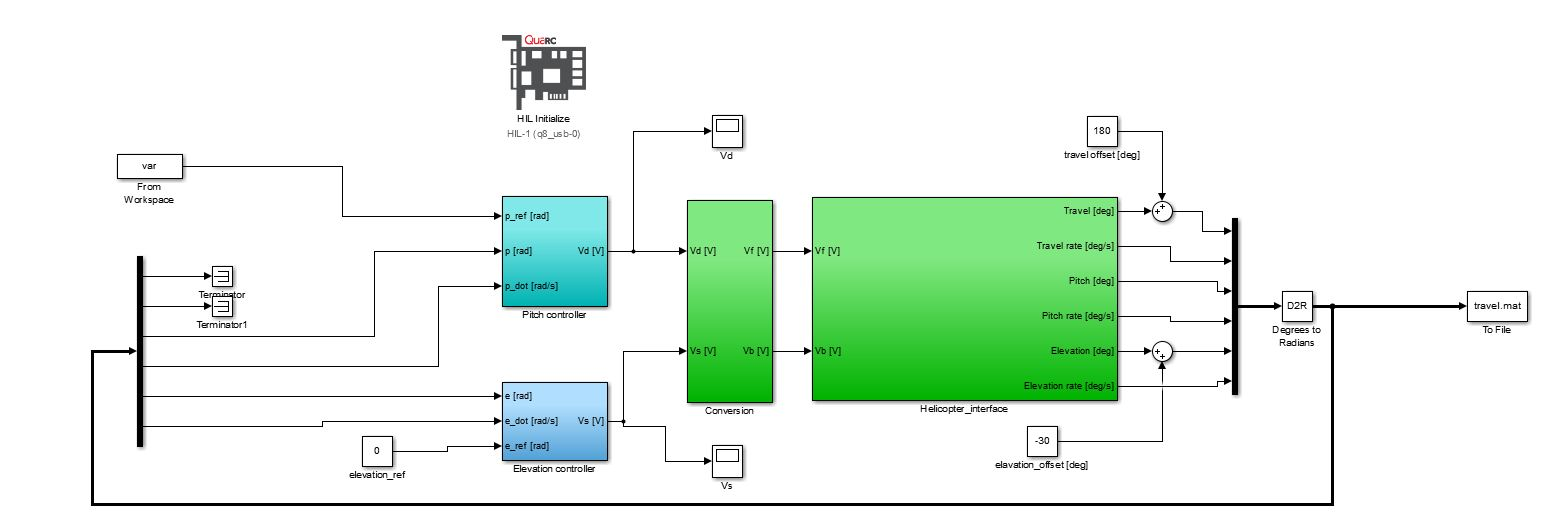
\includegraphics[width=1\linewidth]{figures/simuling_model_1024}
\centering
\caption{Simulink model for optimal control of pitch/travel without feedback}\label{fig:simulink_10_2} 
\end{figure}

Figure \ref{fig:simulink_10_2} shows the Simulink model that is used for this part of the exercise. The figure clearly shows that no feedback is implemented for the optimal input sequence $u^*$ and optimal trajectory $x^*$, which are obtained from the MATLAB-script via the \texttt{From Workspace}-block.

\subsection{Results and discussion}
The calculated trajectories for input ($u$), travel ($\lambda$) and pitch ($p$) for $q = 0.1$, $1$, and $10$ are shown in Figure \ref{fig:10_2_q_0.1}, \ref{fig:10_2_q_1} and \ref{fig:10_2_q_10} below.

\begin{figure}[H]
    \centering
    \captionsetup{justification=centering}
    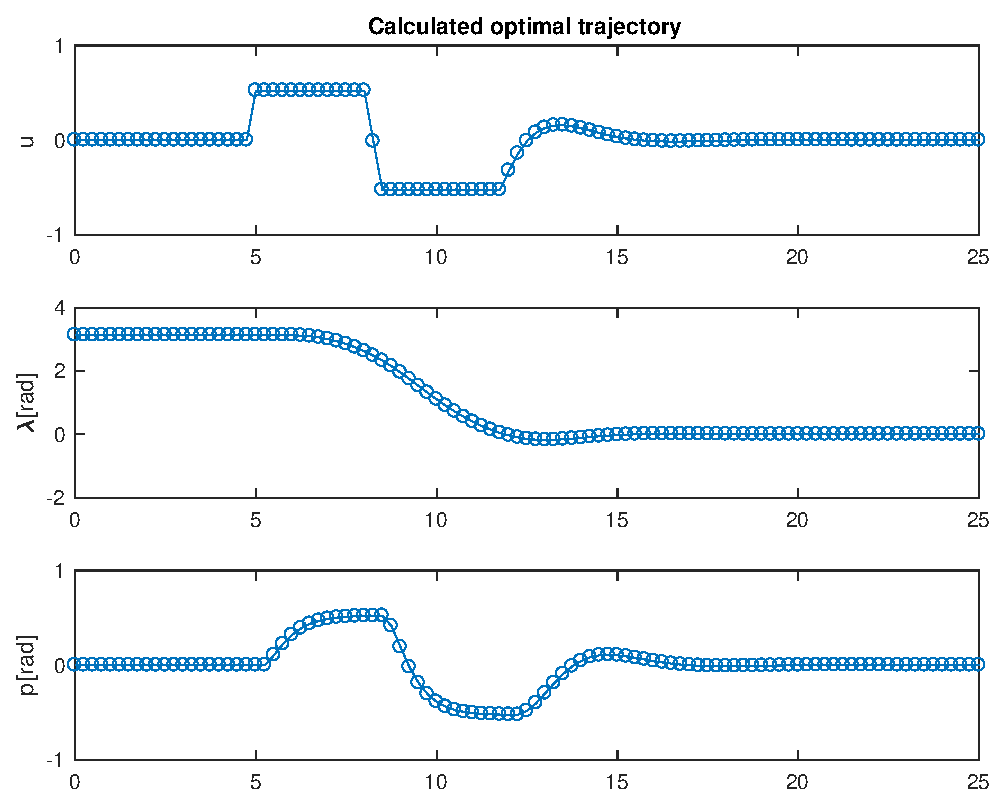
\includegraphics[scale=0.5]{data_10.2/All_states_q_1000000e-01.eps}
    \caption{Calculated optimal trajectory showing input ($u$), travel ($\lambda$) and pitch ($p$) with $q = 0.1$.}
    \label{fig:10_2_q_0.1}
\end{figure}

\begin{figure}[H]
    \centering
    \captionsetup{justification=centering}
    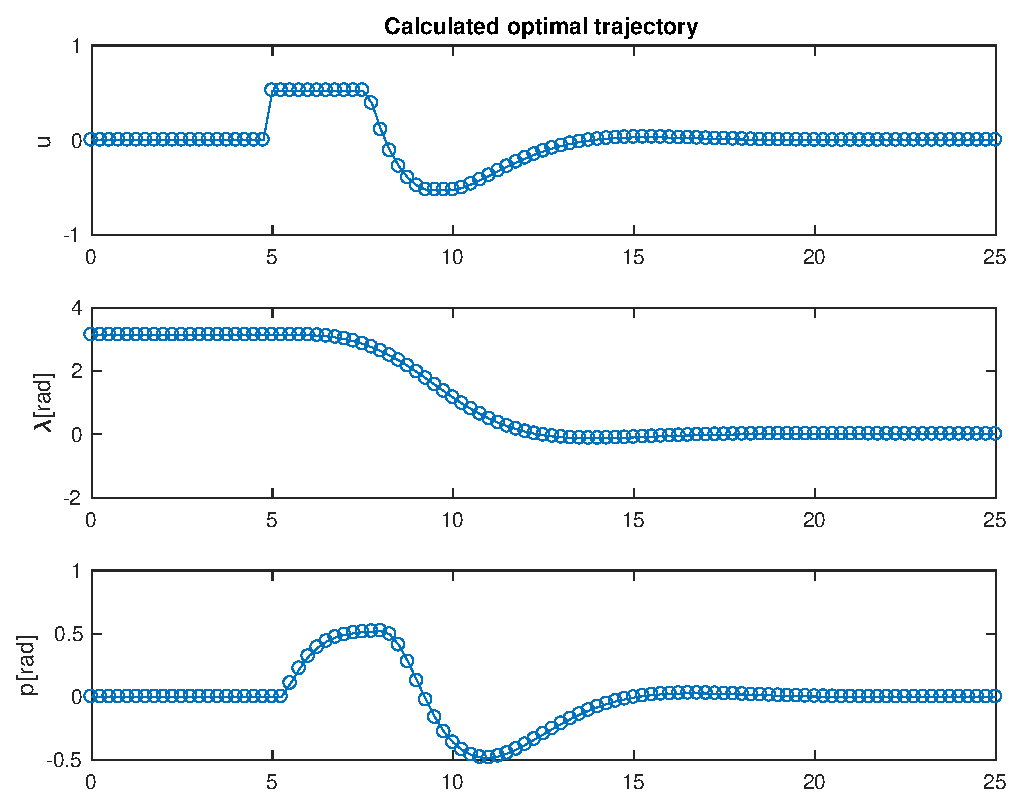
\includegraphics[scale=0.5]{data_10.2/All_states_q_1.eps}
    \caption{Calculated optimal trajectory showing input ($u$), travel ($\lambda$) and pitch ($p$) with $q = 1$.}
    \label{fig:10_2_q_1}
\end{figure}

\begin{figure}[H]
    \centering
    \captionsetup{justification=centering}
    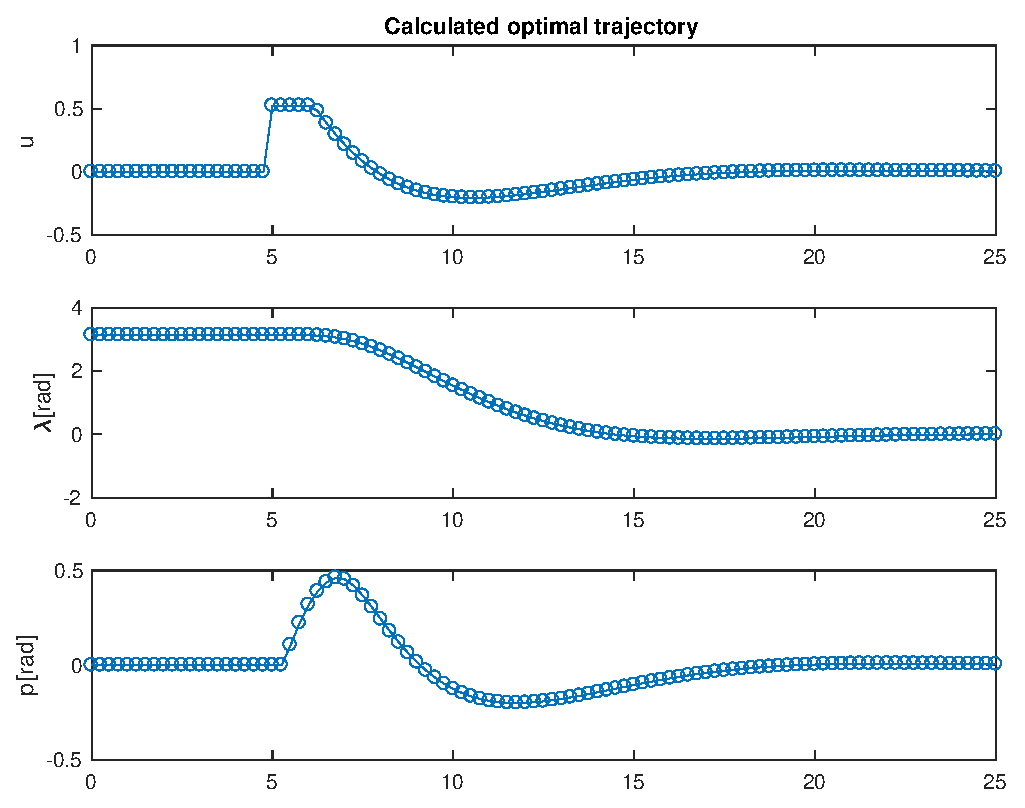
\includegraphics[scale=0.5]{data_10.2/All_states_q_10.eps}
    \caption{Calculated optimal trajectory showing input ($u$), travel ($\lambda$) and pitch ($p$) with $q = 10$.}
    \label{fig:10_2_q_10}
\end{figure}

As seen from the plots in the figures above, increased values of $q$ results in the input $u$ and pitch angle $p$ to maintain its maximum values for shorter periods, which also increases the time it takes for the helicopter to reach its target destination. However, for each value of $q$ both the input $u$ and the pitch angle $p$ reaches its maximum value, allowing for maximum possible speed. The value of $q$ determines how much the pitch angle should be penalized, relative to the state error, ($\lambda_i$ $-$ $\lambda_f$ )$^2$. When calculating an optimal trajectory with a large value of $q$, the pitch will be more penalized, while larger state errors will be allowed. This results in small variations in pitch angle. Likewise, a small value of $q$ will allow for more variation in pitch angle, while state errors will be more penalized. This can be seen from the plots in Figure \ref{fig:10_2_q_0.1}, \ref{fig:10_2_q_1} and \ref{fig:10_2_q_10}.\\

\begin{figure}[H]
\captionsetup{justification=centering}
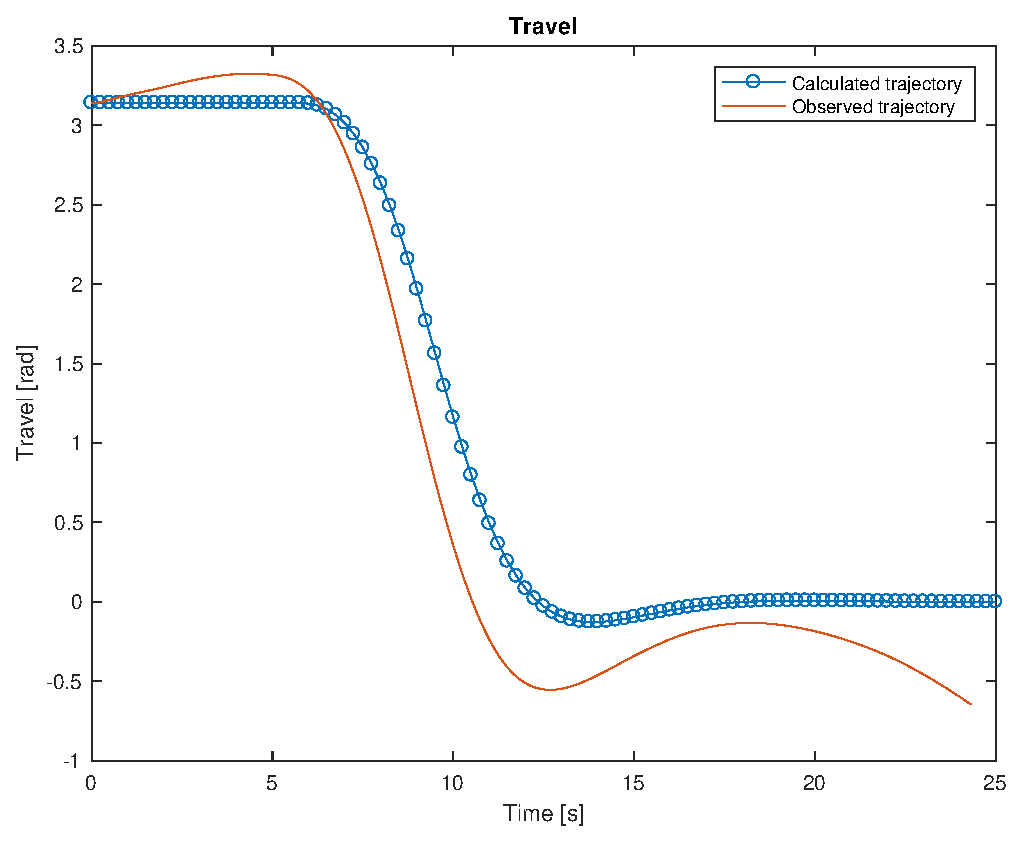
\includegraphics[scale=0.56]{data_10.2/Calculated_vs_Observed_Travel_q_1.eps} 
\centering
\caption{The calculated travel trajectory plotted against the observed travel trajectory with $q = 1$.}  \label{fig:travel_opt}
\end{figure}

\begin{figure}[H]
\captionsetup{justification=centering}
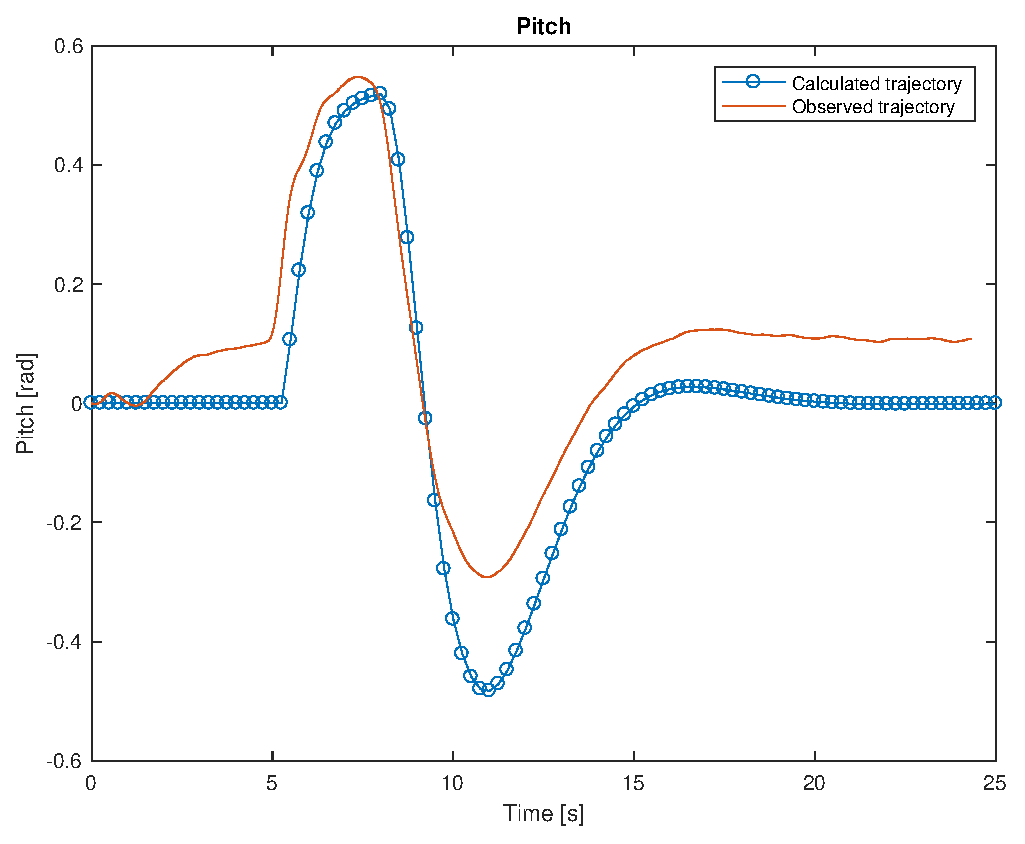
\includegraphics[scale=0.56]{data_10.2/Calculated_vs_Observed_Pitch_q_1.eps} 
\centering
\caption{The calculated pitch trajectory plotted against the observed pitch trajectory with $q = 1$.}
\label{fig:pitch_opt}
\end{figure}

Figure \ref{fig:travel_opt} and \ref{fig:pitch_opt} shows the calculated trajectory for travel and pitch plotted against the measured trajectory for travel and pitch, with $q = 1$. As seen from the plot in Figure \ref{fig:pitch_opt}, the helicopter started off with a small pitch angle, causing it to drift away from $\lambda = \pi$ as shown in Figure \ref{fig:travel_opt}. This means that even with a perfect model and no disturbances, the helicopter would not reach $\lambda = 0$, because the initial point differs from $\lambda = \pi$. However, a perfect system model and no disturbances on the system is unrealistic. A possible solution to this problem would be to implement feedback. This is not done in this section of the exercise, thus the helicopter does not end up in its desired state. Without feedback the helicopter will only follow what was scripted in the MATLAB-file, and with the mentioned imperfect model and disturbances, it is very hard to end up with a good result. 

\section{Optimal Control of Pitch/Travel with Feedback (LQ)}\label{sec:10.3}
\subsection{The Linear Quadratic Regulator} \label{subsec:lqr}
In this section feedback is introduced to our system by implementing a Linear Quadratic Regulator (LQR). The feedback data is obtained by subtracting the calculated optimal states from the measured states. If a deviation occurs, the controller compensates by altering the control input $u_{k}$, given by
\begin{equation}\label{eq:feedBackGain}
u_{k} = u_{k}^*-K^\top(x_{k}-x_{k}^*)
\end{equation}

\begin{figure}[H]
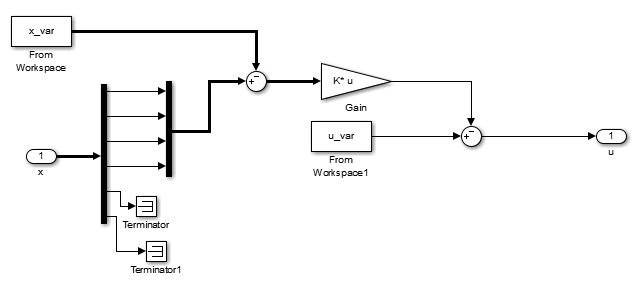
\includegraphics[width=1\linewidth, height=7cm]{figures/LQR_model} 
\centering
\caption{Simulink diagram of the Linear Quadratic Controller}\label{fig:figur7}
\end{figure}

The LQR is implemented in Simulink and an optimal gain matrix $K$ is found by using the MATLAB function \texttt{dlqr}, which calculates $K$ by using the infinite horizon solution $S$ of the associated discrete-time Riccati equation \cite{MathWorks}:

\begin{equation}\label{eq:gainMatrix}
K = (B^\top SB+R)^{-1}(B^\top SA)
\end{equation}

This modification leads to a change in the control hierachy, illustrated in Figure \ref{fig:figur8}.

\begin{figure}[H]
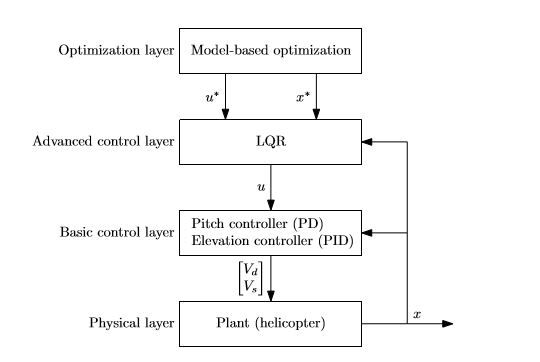
\includegraphics[width=1\linewidth, height=7cm]{figures/10_3ControlHieraky} 
\centering
\caption{Updated hiearchy with LQR}\label{fig:figur8}
\end{figure}\\

The quadratic function to be minimized by the controller is

\begin{subequations}\label{eq:10_3_linmod}
\begin{equation}\label{eq:10_3_objfunc}
J = \sum_{i=0}^{\infty} \triangle x_{i+1}^\top Q_{lqr} \triangle x_{i+1}+\triangle u_{i}^\top R_{lqr} \triangle u_{i},\quad Q_{lqr}\geq 0,\quad R_{lqr}>0
\end{equation}
\begin{equation}
\triangle x_{i+1} = A\triangle x_{i} + B\triangle u_{i} \end{equation}
\begin{equation}
\triangle x = x - x^*        
\end{equation}
\begin{equation}
\triangle u = u - u^*        
\end{equation}		
\end{subequations}

where $Q_{lqr}$ and $R_{lqr}$ are diagonal matrices that are used to penalize deviation in the states or in the feedback variable $u_{k}$.

\newpage
\subsection{Results and discussion}
The system was implemented and tested with different values of Q and R, focusing on travel. Satisfactory results were found by adding a small penalty on the input deviations, making the helicopter react faster. 

\begin{equation}
{Q_{lqr}} = \left[ {\begin{array}{*{20}{c}}
{1}&0&0&0\\
0&0&0&0\\
0&0&0&0\\
0&0&0&0
\end{array}} \right],\quad {R_{lqr}} = 0.1
\end{equation}


\begin{figure}[H]
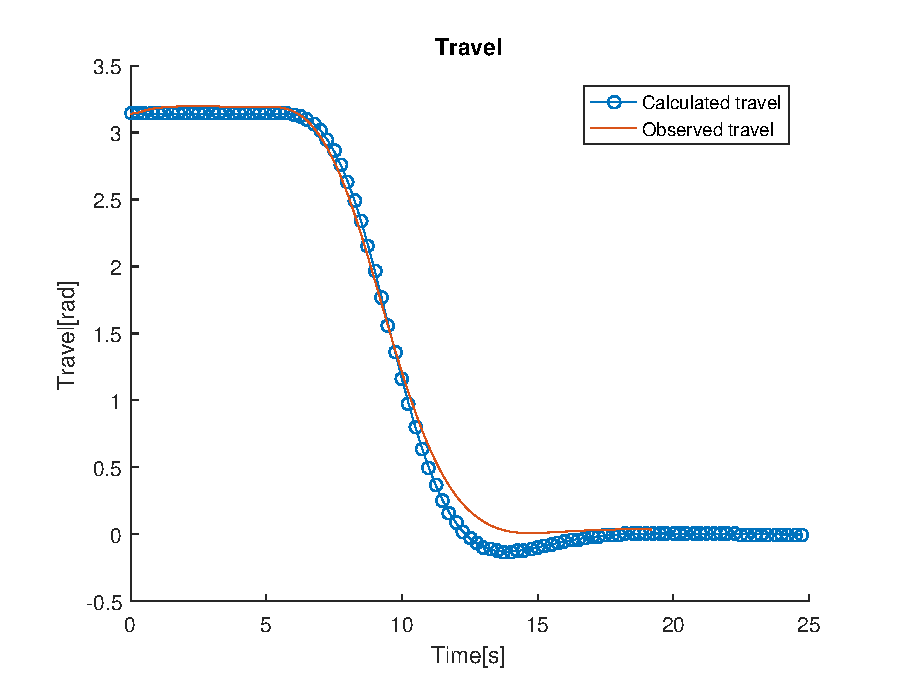
\includegraphics[scale=0.73]{data_10.3/10_3_travel_opt_and_observed} 
\centering
\caption{Observed travel ($\lambda$) compared to calculated trajectory}\label{fig:figur9}
\end{figure}

\begin{figure}[H]
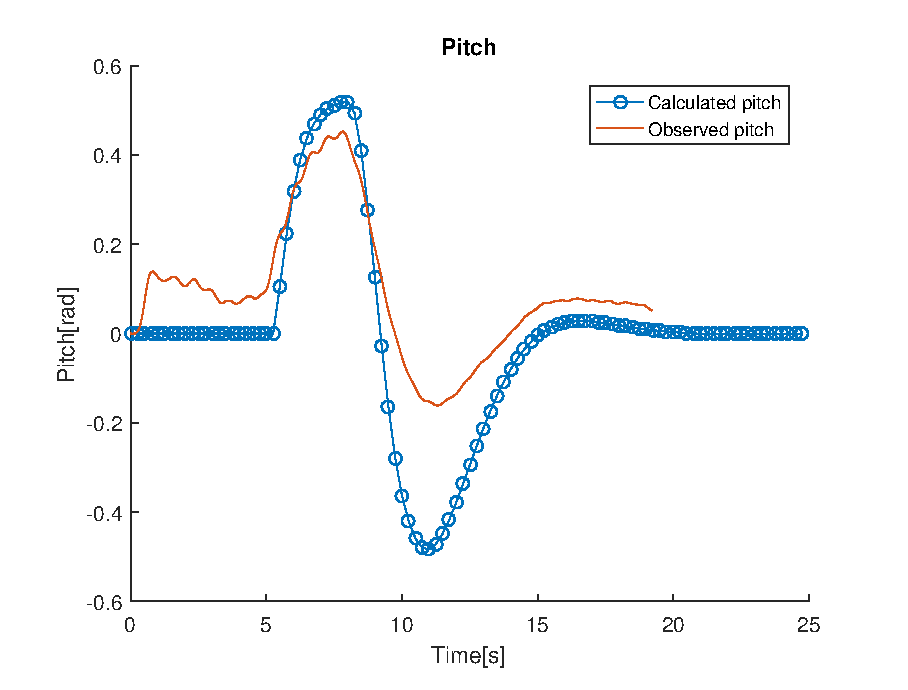
\includegraphics[scale=0.73]{data_10.3/10_3_pitch_opt_and_observed} 
\centering
\caption{Observed pitch ($p$) compared to calculated values}\label{fig:figur9}
\end{figure}

As seen from figure 11 and 12, the measured travel follows the calculated trajectory quite well, while the measured pitch has slight deviations. As seen in the case without feedback in Section \ref{sec:10.2}, the helicopter starts drifting away after it has reached its desired destination. It also starts off with a small pitch angle. This does not happen in this section, meaning that feedback can be used as a utility to compensate for disturbances and model inaccuracies. 

\subsubsection{Alternative control strategies}
Instead of using an LQ controller, Model Predictive Control (MPC) could be used. MPC would be implemented by using the current state as the initial value and solving an open-loop optimal control problem at each time step, over a specified time interval. The first control in the output sequence is then applied to the system and the process repeats itself. A disadvantage compared to the LQR case is that it costs more computationally. In addition, the performance of an MPC is highly dependent on having well tuned PID controllers in the control layer. In this lab it might be wise to retune the controllers to ensure that this is the case before implementation of an MPC. It is also important that the physical model is as accurate as possible. Given this, an MPC would most likely give better performance with better reference tracking and disturbance rejection compared to an LQR.   \cite{Foss2016} 






\section{Optimal Control of Pitch/Travel and Elevation with and without Feedback}\label{sec:10.4}

Previously this report has only been focusing on optimal control of pitch and travel, calculating an optimal trajectory without considering elevation. This will be done in this section. In addition, nonlinear constraints are also added to the optimization problem. 

\subsection{Continous state space form}

By adding elevation $e$ and elevation rate $\dot{e}$ to the state vector, the model can be written on continuous state space form

\begin{equation}
\begin{aligned}
$$\dot{x} = {A_c}x + {B_c}u$$      
\end{aligned}
\end{equation}

where $x = \left[ {\begin{array}{*{20}{r}}\lambda &r&p&{\dot{p}}&e&{\dot{e}} \end{array}}\right]^\top$ and $u = [ {\begin{array}{*{20}{c}}p_c&u_c\end{array}}]^\top$. The system matrices $A_c$ and $B_c$ are given by

\begin{equation}
\begin{aligned}
    $$A_c = \left[ {\begin{array}{*{20}{c}}
0&1&0&0&0&0\\
0&0&{ - {K_2}}&0&0&0\\
0&0&0&1&0&0\\
0&0&{ - {K_1}{K_{pp}}}&{ - {K_1}{K_{dp}}}&0&0\\
0&0&0&0&0&1\\
0&0&0&0&{ - {K_3}{K_{ep}}}&{ - {K_3}{K_{ed}}}
\end{array}} \right]$$
\end{aligned}
\end{equation}


\begin{equation}
\begin{aligned}
$$B_c = \left[ {\begin{array}{*{20}{c}}
0&0\\
0&0\\
0&0\\
{{K_1}{K_{pp}}}&0\\
0&0\\
0&{{K_3}{K_{ep}}}
\end{array}} \right]$$
\end{aligned}
\end{equation}

\subsection{Discretized State Space Model}

The model is discretized by using the Forward Euler Method as in Section \ref{sec:10.2}, given by Equation \ref{eq:forwardeuler}.
Thus, the model can be written on discrete time state space form

\begin{equation}
\begin{aligned}
$${x_{k + 1}} = A{x_k} + B{u_k}$$
\end{aligned}
\end{equation}

where $A$ and $B$ are given by

\begin{equation}
$$A = I + \Delta t{A_c}=\left[ {\begin{array}{*{20}{r}}
  1&\Delta t&0&0&0&0 \\ 
  0&1&{ - \Delta t{K_2}}&0&0&0 \\ 
  0&0&1&h&0&0 \\ 
  0&0&{ - \Delta t{K_1}{K_{pp}}}&{1 - \Delta t{K_l}{K_{dp}}}&0&0 \\ 
  0&0&0&0&1&\Delta t \\ 
  0&0&0&0&{ - \Delta t{K_3}{K_{ep}}}&{1 - \Delta t{K_3}{K_{ed}}} 
\end{array}} \right]$$
\end{equation}\\

\begin{equation}
\begin{aligned}
$$B = \Delta t{B_c} = \left[ {\begin{array}{*{20}{r}}
  0&0 \\ 
  0&0 \\ 
  0&0 \\ 
  {\Delta t{K_1}{K_{pp}}}&0 \\ 
  0&0 \\ 
  0&{\Delta t{K_3}{K_{ep}}} 
\end{array}} \right]$$
\end{aligned}
\end{equation}



\subsection{Optimization problem with new nonlinear constriants}

In this section, as the previous, the objective is to calculate an optimal trajectory from 
${x_0}=[{\lambda_0}\quad 0\quad 0\quad 0 \quad 0\quad 0]^\top$ to 
${x_f}=[{\lambda_f}\quad 0\quad 0\quad 0 \quad 0\quad 0]^\top$

This trajectory is calculated by minimizing the objective function
\begin{equation}
\begin{aligned}
$$\phi  = \sum\limits_{i = 1}^N {{{({\lambda _i} - {\lambda _f})}^2} + {q_1}p_{ci}^2 + {q_2}e_{ci}^2} $$
\end{aligned}
\end{equation}

which is a quadratic objective function that can be reformulated by using equation (4.11) from \cite{Foss2016},
\begin{equation}
\begin{aligned}
$$\phi  = \sum\limits_{i = 0}^{N-1} {(x_{i+1}-x_{i+1}^{ref})^\top Q(x_{i+1}-x_{i+1}^{ref}) + u_t^\top Ru_t} $$
\end{aligned}
\end{equation}

where 

$$Q = \left[ {\begin{array}{*{20}{c}}
  1&0&0&0&0&0 \\ 
  0&0&0&0&0&0 \\ 
  0&0&0&0&0&0 \\ 
  0&0&0&0&0&0 \\ 
  0&0&0&0&0&0 \\ 
  0&0&0&0&0&0 
\end{array}} \right],R = \left[ {\begin{array}{*{20}{c}}
  {{q_1}}&0 \\ 
  0&{{q_2}} 
\end{array}} \right]$$

In addition to the equality constraints from previous sections, a nonlinear inequality constraint is added on the elevation. To calculate this nonlinear inequality constraint, a function in MATLAB is created and added in the built-in function for calculating the optimal trajectory. The nonlinear inequality constraint added is

\begin{equation}
\begin{aligned}
$${e_k} \ge \alpha \exp ( - \beta {({\lambda _k} - {\lambda _t})^2}) \quad  \forall k \in \{ 1,...,N\} $$
\end{aligned}
\end{equation}

which in order to be implemented in the built-in function is reformulated as
\begin{equation}
\begin{aligned}
$$c({x_k}) = \alpha \exp ( - \beta {({\lambda _k} - {\lambda _t})^2}) - {e_k} \le 0$$
\end{aligned}
\end{equation}

with $\alpha = 0.2$, $\beta = 20$ and $\lambda_k = \frac{2\pi}{3}$.
Both of these functions are passed into the MATLAB-function \texttt{fmincon}, which calculates the optimal trajectory for the helicopter. $\Delta t = 0.25 $ and $N = 40$ are used, which yields an optimizing horizon of 10 seconds.

With the equality constraints from previous sections and the new nonlinear constraint, the optimization problem can be stated as

\begin{subequations}
    \begin{equation}
    \begin{aligned}
        $$\mathop {\min }\limits_z  = {z^\top}Gz$$
    \end{aligned}
    \end{equation}
    subject to
        \begin{equation}
    \begin{aligned}
        $$ A$_{eq}$z = b$_{eq}$ $$
    \end{aligned}
    \end{equation}
    \begin{equation}
    \begin{aligned}
        $$c({x_k}) \le 0$$
    \end{aligned}
    \end{equation}
    \begin{equation}
    \begin{aligned}
        $$p_{min} \le p_k \le p_{max}$$
    \end{aligned}
    \end{equation}
\end{subequations}

It is worth noting that the default optimizing algorithm in MATLAB did not converge to an optimal solution. It was therefore necessary to use the SQP (Sequential Quadratic Programming) algorithm to solve the optimization problem.

\subsection{Compare results with and without feedback}\label{subsec:feedback}

The optimal input sequence calculated using the new cost function and constraints is implemented in Simulink, first simulated without using feedback. For simulation with feedback, the LQR is implemented as in subsection~\ref{subsec:lqr} and now with all the states connected,

$${Q_{lqr}} = \left[ {\begin{array}{*{20}{c}}
  1&0&0&0&0&0 \\ 
  0&1&0&0&0&0 \\ 
  0&0&1&0&0&0 \\ 
  0&0&0&1&0&0 \\ 
  0&0&0&0&1&0 \\ 
  0&0&0&0&0&1 
\end{array}} \right],{R_{lqr}} = \left[ {\begin{array}{*{20}{c}}
  1&0 \\ 
  0&1 
\end{array}} \right]$$

Different values for $Q_{lqr}$ and $R_{lqr}$ are experimented with to obtain a more smooth and even trajectory for the helicopter. 

\subsubsection{Decoupled states}
In this model, the elevation $e$ and elevation rate $\dot{e}$ is completely decoupled from the other states. This does not fit well with reality. At small pitch angles, elevation is mostly dependent on pitch, but at larger pitch angles the travel rate and elevation rate is dependent variables. This simplification of the model yields an offset in the solution. Coupling all the states together would provide a more precise, but also a more complex model.

\subsection{Optional: More constraints}\label{subsec:constraints}

With the optimal trajectory calculated by minimizing the objective function, the helicopter went slightly beyond $\lambda_f = \pi$ before it turned back and stabilized at $\lambda_f$. Hence, it was tempting to try adding other constraints on the objective function. Constraining the elevation rate $\dot{e}$, and velocity (travel rate) $\dot{\lambda}$, should produce a different result that may prevent the overshoot.
\begin{table}[H]
\centering
\label{constraints}
\renewcommand{\arraystretch}{1.1}
\caption{Additional constraints}
\begin{tabular}{lll}
\toprule
Constraint    &    $\dot{\lambda}$        & $\dot{e}$ \\
\midrule
1             & $\frac{-20\pi}{180} - \frac{5\pi}{180}$  & $\frac{-\pi}{180} - 0$                   \\
2             & $\frac{-5\pi}{180} - \frac{5\pi}{180}$ & $\frac{-\pi}{180} - \frac{10\pi}{180}$   \\
3             & $\frac{-5\pi}{180} - \frac{5\pi}{180}$ & $\frac{-\pi}{180} - \frac{10\pi}{180}$   \\
4             & $\frac{-10\pi}{180} - \frac{10\pi}{180}$ & $\frac{-5\pi}{180} - \frac{5\pi}{180}$   \\
5             & - & -   \\
\bottomrule
\end{tabular}
\end{table}

Very strict constraints on the objective function results in the SQP-algorithm not converging to an optimal solution. It was therefore necessary to loosen the constraints. All the constraints, except the third, were simulated with 40 time steps. The third constraint were simulated using 80 time steps. 

\subsection{Results and discussion}
This subsection will present and discuss the results from the previous subsections.
\subsubsection{Without feedback}
The optimal trajectory calculated using the new objective function and nonlinear constraints was first simulated without feedback.

\begin{figure}[H]
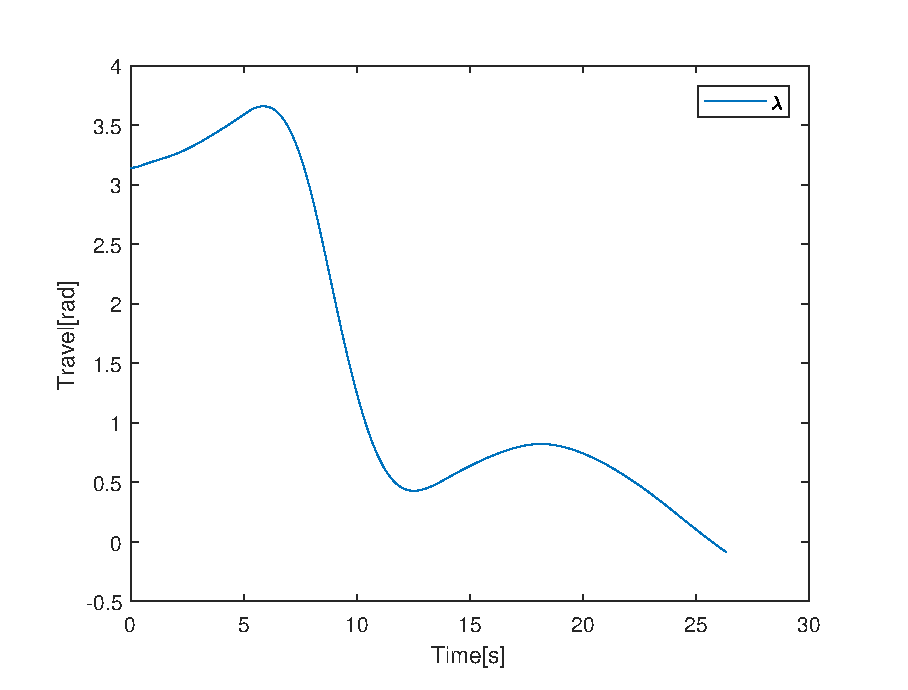
\includegraphics[width=1\linewidth, height=7cm]{data_10.4/travel_uten_feedback_eps.eps} 
\centering
\caption{Observed travel without feedback}\label{fig:travelufeedback}
\end{figure}

\begin{figure}[H]
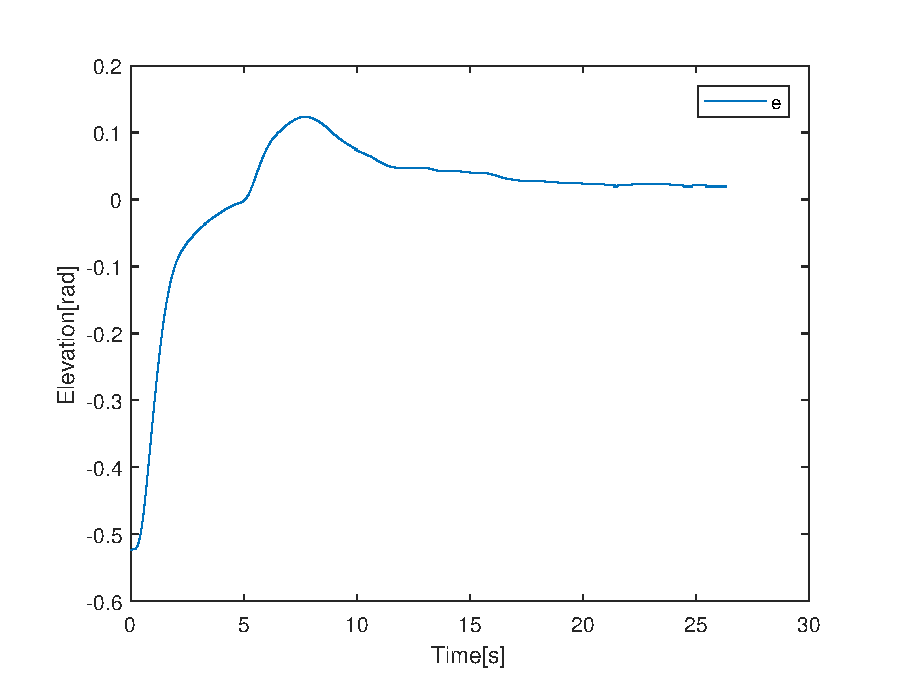
\includegraphics[width=1\linewidth, height=7cm]{data_10.4/elevation_uten_feedback_eps.eps} 
\centering
\caption{Observed elevation without feedback}\label{fig:elevationufeedback}
\end{figure}

Figure~\ref{fig:travelufeedback} and Figure~\ref{fig:elevationufeedback} shows the helicopters trajectory when simulating without feedback. The helicopter drifted away from the start point which lead to the helicopter not stopping at $\lambda = 0$. After 15 seconds the output was set to zero, which explains why the helicopter drifted away from the desired position. There were no significant differences on the observed elevation with and without feedback. As shown in figure~\ref{fig:elevationufeedback}, the observed elevation does not differ much from the optimization. 

\subsubsection{With feedback}

Feedback was again implemented as presented in subsection~\ref{subsec:feedback}. The feedback gain matrix $K$ was adjusted by changing the weights in the $Q_{lqr}$ and $R_{lqr}$ matrix. 

\begin{figure}[H]
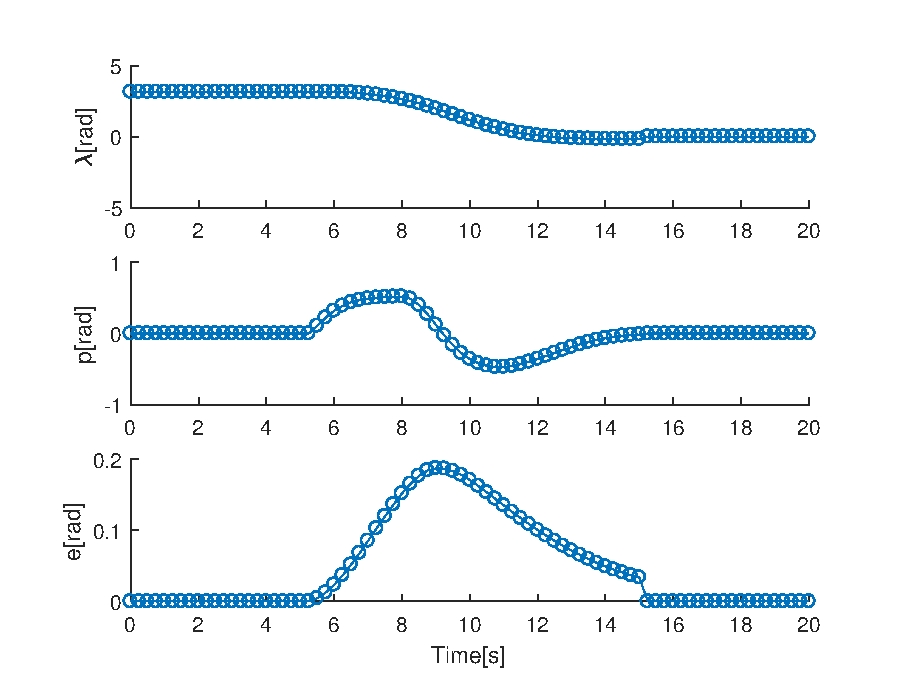
\includegraphics[width=1\linewidth, height=8cm]{data_10.4/states_eps.eps} 
\centering
\caption{The calculated optimal trajectory showing travel, $\lambda$, pitch, $p$, and elevation, $e$.}\label{fig:states_1}
\end{figure}

Figure~\ref{fig:states_1} shows the calculated optimal trajectory for travel $\lambda$, pitch $p$, and elevation $e$. In comparison with   Section~\ref{sec:10.3}, the introduction of the two new states and the nonlinear constraint on elevation is clearly visible as the elevation now has a distinct trajectory. 

\begin{figure}[H]
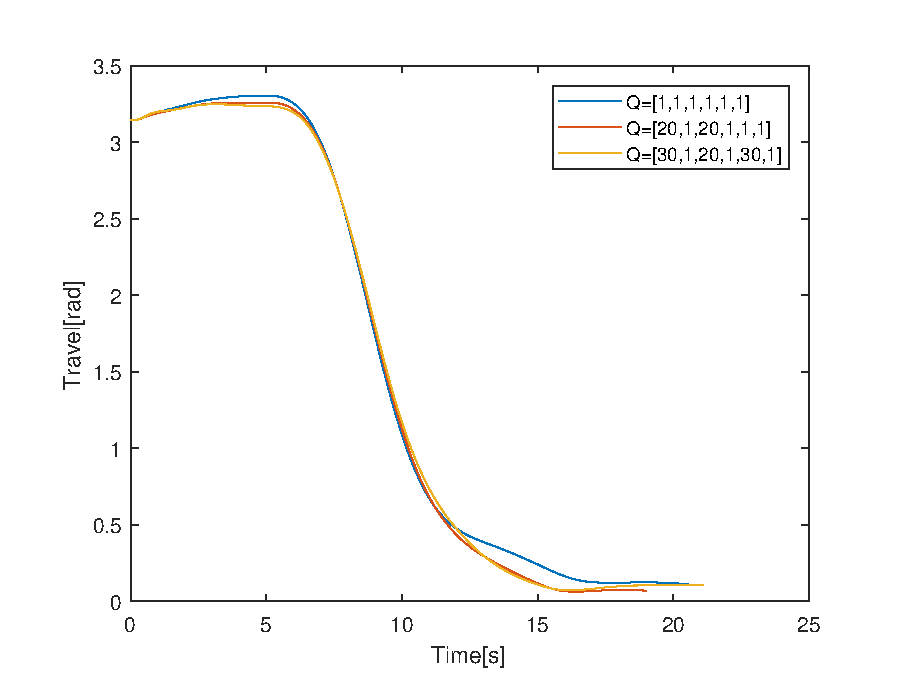
\includegraphics[width=1\linewidth, height=8cm]{data_10.4/travel_eps.eps} 
\centering
\caption{Observed travel with three different Q matrices}\label{fig:travel1}
\end{figure}

\begin{figure}[H]
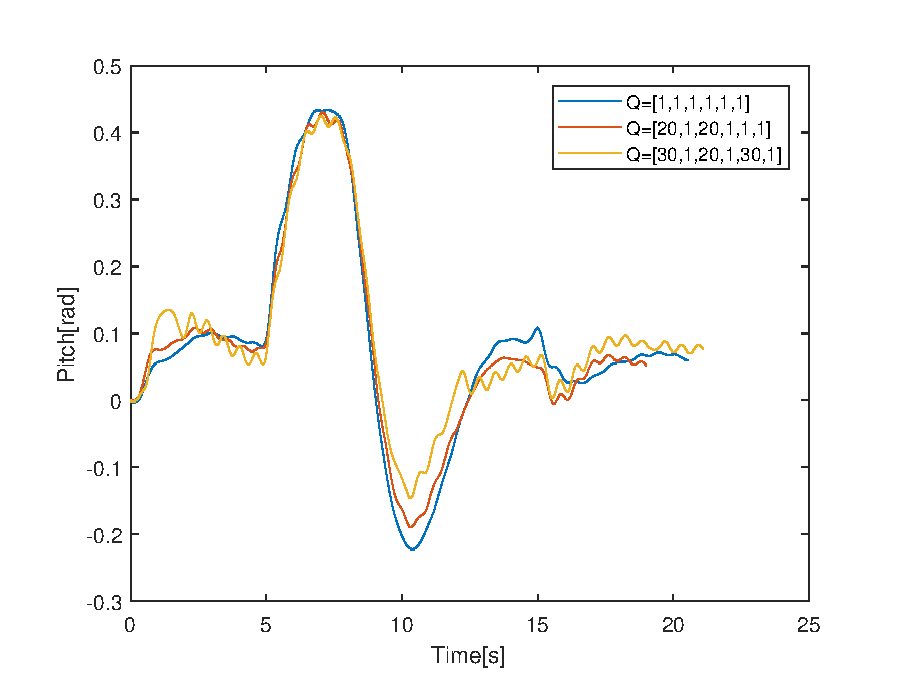
\includegraphics[width=1\linewidth, height=8cm]{data_10.4/pitch_eps.eps} 
\centering
\caption{Observed pitch with three different Q matrices}\label{fig:pitch1}
\end{figure}

\begin{figure}[H]
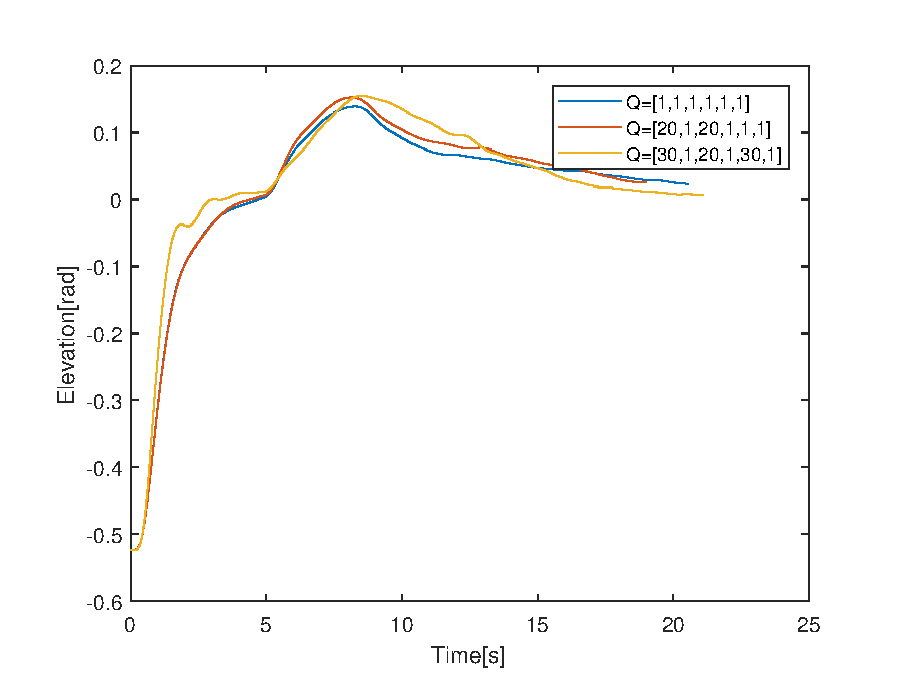
\includegraphics[width=1\linewidth, height=8cm]{data_10.4/elevation_eps.eps} 
\centering
\caption{Observed elevation with three different Q matrices}\label{fig:elevation1}
\end{figure}

Figure~\ref{fig:travel1}, ~\ref{fig:pitch1} and ~\ref{fig:elevation1} shows how the helicopter performs with respect to travel, pitch and elevation. In each graph, the $K$ matrix was calculated using three different Q matrices, where the diagonals were $[\begin{matrix}
   1 & 1 & 1 & 1 & 1 & 1\end{matrix}]$, $[\begin{matrix}
   20 & 1 & 20 & 1 & 1 & 1\end{matrix}]$ and $[\begin{matrix}
   30 & 1 & 20 & 1 & 30 & 1\end{matrix}]$ with the diagonal of $R$ being $[\begin{matrix}1 & 1\end{matrix}]$ for all three Q matrices. 
It is evident, as expected, that the weighing on the different states has an impact on how the helicopter behaves, but it does not have a significant impact on the observed travel. The resulting travel from the three different cases does not differ much, there is some differences in the time to convergence, but all three follow a similar trajectory. 
In regard to pitch, increased weights introduced more small oscillations, but it also decreased the larger oscillations. Neglecting the small oscillations, the pitch is very similar to the calculated pitch in figure~\ref{fig:states_1}.
The observed elevation for the three different cases is, as for the travel, no significant difference compared to the optimization. The second case has a slightly lower decrease in elevation.

\subsubsection{Additional constraints}
In order to study the affect of constraining different states, constraints as described in \ref{subsec:constraints} were introduced to the optimization problem.

\begin{figure}[H]
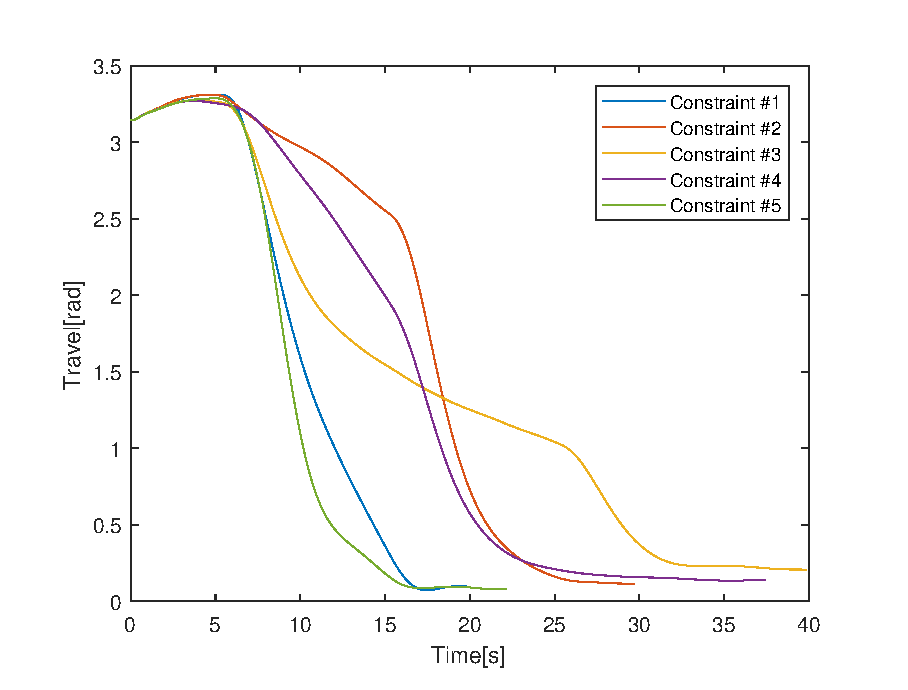
\includegraphics[width=1\linewidth, height=8cm]{data_10.4/constraints_eps.eps} 
\centering
\caption{Observed travel with five different constraints as described in \ref{subsec:constraints}}\label{fig:ctravel}
\end{figure}

The observed travel for the five different constraints displays a good representation of the high consequence of strict constraints. The first and fifth constraint are fairly similar, except slight difference at the end of simulation. The second, third and fourth constraint are significantly slower than the two other. The second and third (which was simulated with 80 time steps) constraint did not converge to an optimal solution, and the simulation of the two displayed an odd behaviour with respect to travel rate. This is observable in figure~\ref{fig:ctravel} after about 20 and 30 seconds respectively. 

\begin{figure}[H]
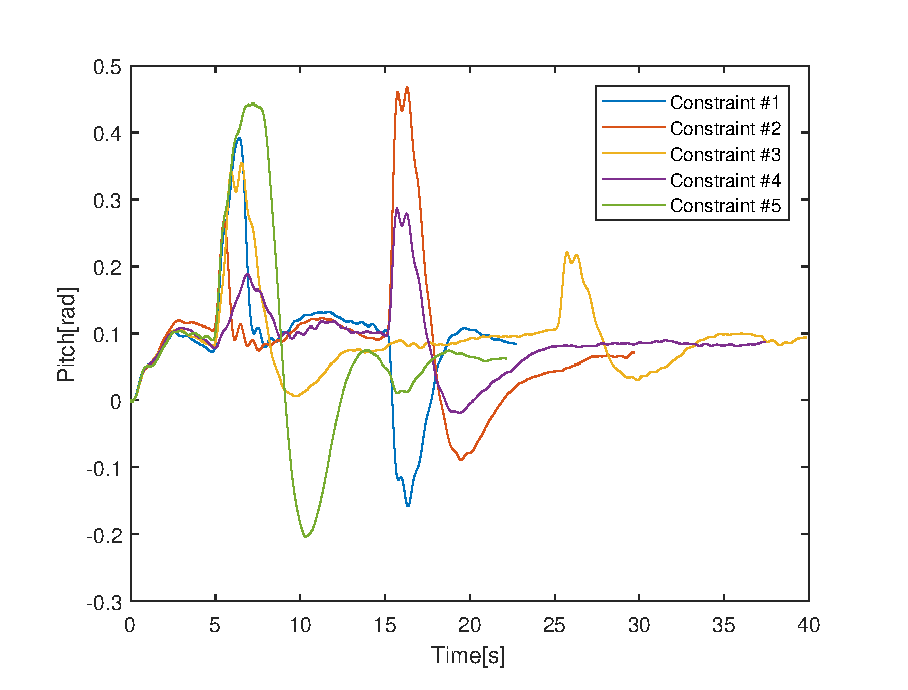
\includegraphics[width=1\linewidth, height=8cm]{data_10.4/constraints_p_eps.eps} 
\centering
\caption{Observed pitch with constraints}\label{fig:cpitch}
\end{figure}

With the new constraints there was a big difference in the observed pitch for the five cases. Compared to the observed travel, they correspond well to how the helicopter behaved, where high differences in pitch leads to high travel rate. 

\begin{figure}[H]
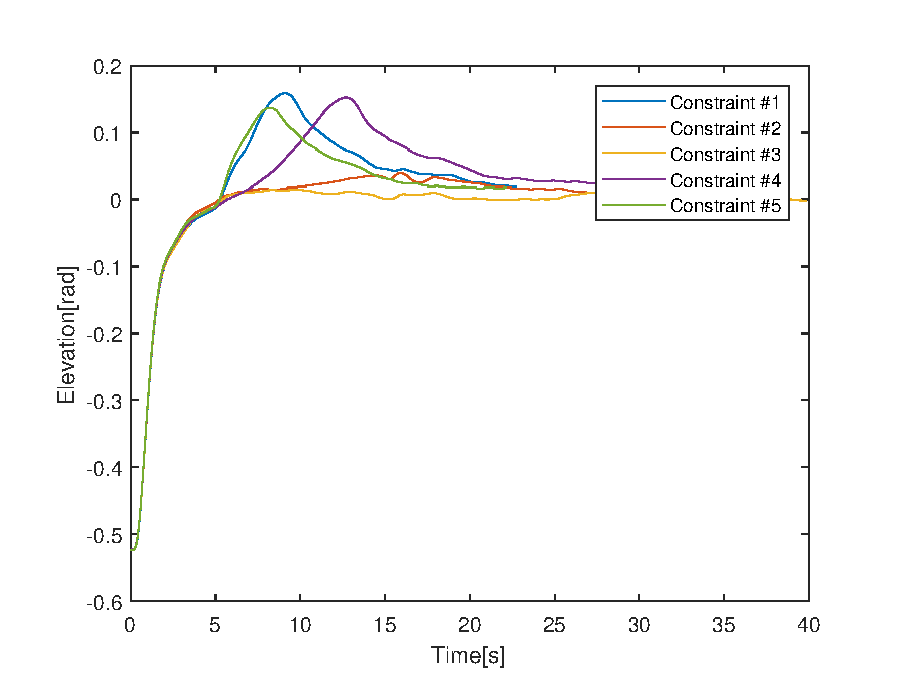
\includegraphics[width=1\linewidth, height=8cm]{data_10.4/constraints_e_eps.eps} 
\centering
\caption{Observed elevation with constraints}\label{fig:celev}
\end{figure}

For the first three cases the observed elevation is very similar, as expected with the strict constraints on elevation rate. The fourth constraint, where the elevation rate had more room to manoeuvre in, yielded a similar behaviour as previous simulations. 

\subsubsection{Discussion}
With the introduction of elevation to the system states, the optimization problem now included a new dimension, elevation. In section~\ref{sec:10.3} the helicopter had a nearly constant elevation, where the optimization problem focused on the first four states. With the elevation included, the helicopter now behaved more naturally, neglecting the unrealistic decoupled states, with an the elevation being dependent on pitch and travel rate.

For the simulation without feedback, the helicopter behaved as expected, with a slight overshoot, before drifting away from the desired $\lambda$ value. The observed elevation was very similar to the calculated elevation. The behaviour of the helicopter may be improved with a better tuning of the regulators, but as this was not the scope of this report we did not prioritize this.

With feedback and LQR implemented again, a series of different weights on the $Q_{lqr}$ and $R_{lqr}$ were tested. As presented, the resulting travel, pitch and elevation did not differ much. We expected a bigger difference in the behaviour, especially with respect to travel and pitch. The LQR corrects the trajectory and does not let the helicopter deviate much from the calculated optimal trajectory. The three cases in figure~\ref{fig:travel1}, ~\ref{fig:pitch1} and ~\ref{fig:elevation1} does not differ much from the calculated trajectory presented in figure~\ref{fig:states_1}. It is also worth noting that we experienced some technical problems with the QuaRC encoder during these tests, as was reported to the learning assistants. These problems, which were present occasionally, may have influenced the results. 
The additional constraints clearly showed the huge difference strict constraints have on the optimization problem. The four additional constraints added were not meant to give a "better" performance, but to give a brief overview of how the constraints affect the solution to the problem. With very strict constraints as in constraint two and three, the algorithm did not converge to an optimal solution. This was clearly visible in figure~\ref{fig:ctravel}, as constraint two and three had an odd travel at the end of simulation. With a more defined task, these additional constraints may provide a behaviour that is more satisfying.
\include{EndResultsAndDiscussion}
\section{Conclusion}\label{sec:conclusion}
The optimal trajectory for the helicopter is achieved by using some of the built-in functions in MATLAB to minimize the objective function. The results from these calculations were satisfying, and with the introduction of feedback and LQR the helicopter did not drift away from the desired position. Additional constraints may be added to give the helicopter a more accurate performance. All in all, the performance of the implemented tools and calculations are shown by several tests to yield a satisfying result.
\addcontentsline{toc}{section}{Appendix} % Remove this if you don't want the appendix included in the table of contents.
\appendix

\section{MATLAB Code}\label{sec:matlab}

These MATLAB codes does not contain all the code from the project, but the necessary code to solve the different problems. Subsection~\ref{subsec:10_2_m} and ~\ref{subsec:10_3_m} build on the same theory and therefore subsection~\ref{subsec:10_2_m} contain some of the code needed in problem 10.3. The last subsection contain the code for the nonlinear constraint for problem 10.4.

\subsection{oppg10\_2.m}\label{subsec:10_2_m}
\lstinputlisting{code/oppg10_2.m}
\subsection{oppg10\_3.m}\label{subsec:10_3_m}
\lstinputlisting{code/oppg10_3.m}
\subsection{oppg10\_4.m}\label{subsec:10_4_m}
\lstinputlisting{code/oppg10_4.m}
\subsection{nonlconst.m}\label{subsec:nonlconst_m}
\lstinputlisting{code/nonlconst.m}

\section{Simulink Diagrams}\label{sec:simulink}
The two first Simulink diagrams are presented in sections~\ref{sec:10.2} and ~\ref{sec:10.3}. Hence, only the simulink diagrams for problem 10.4 is presented here.

\begin{figure}[H]
    \centering
    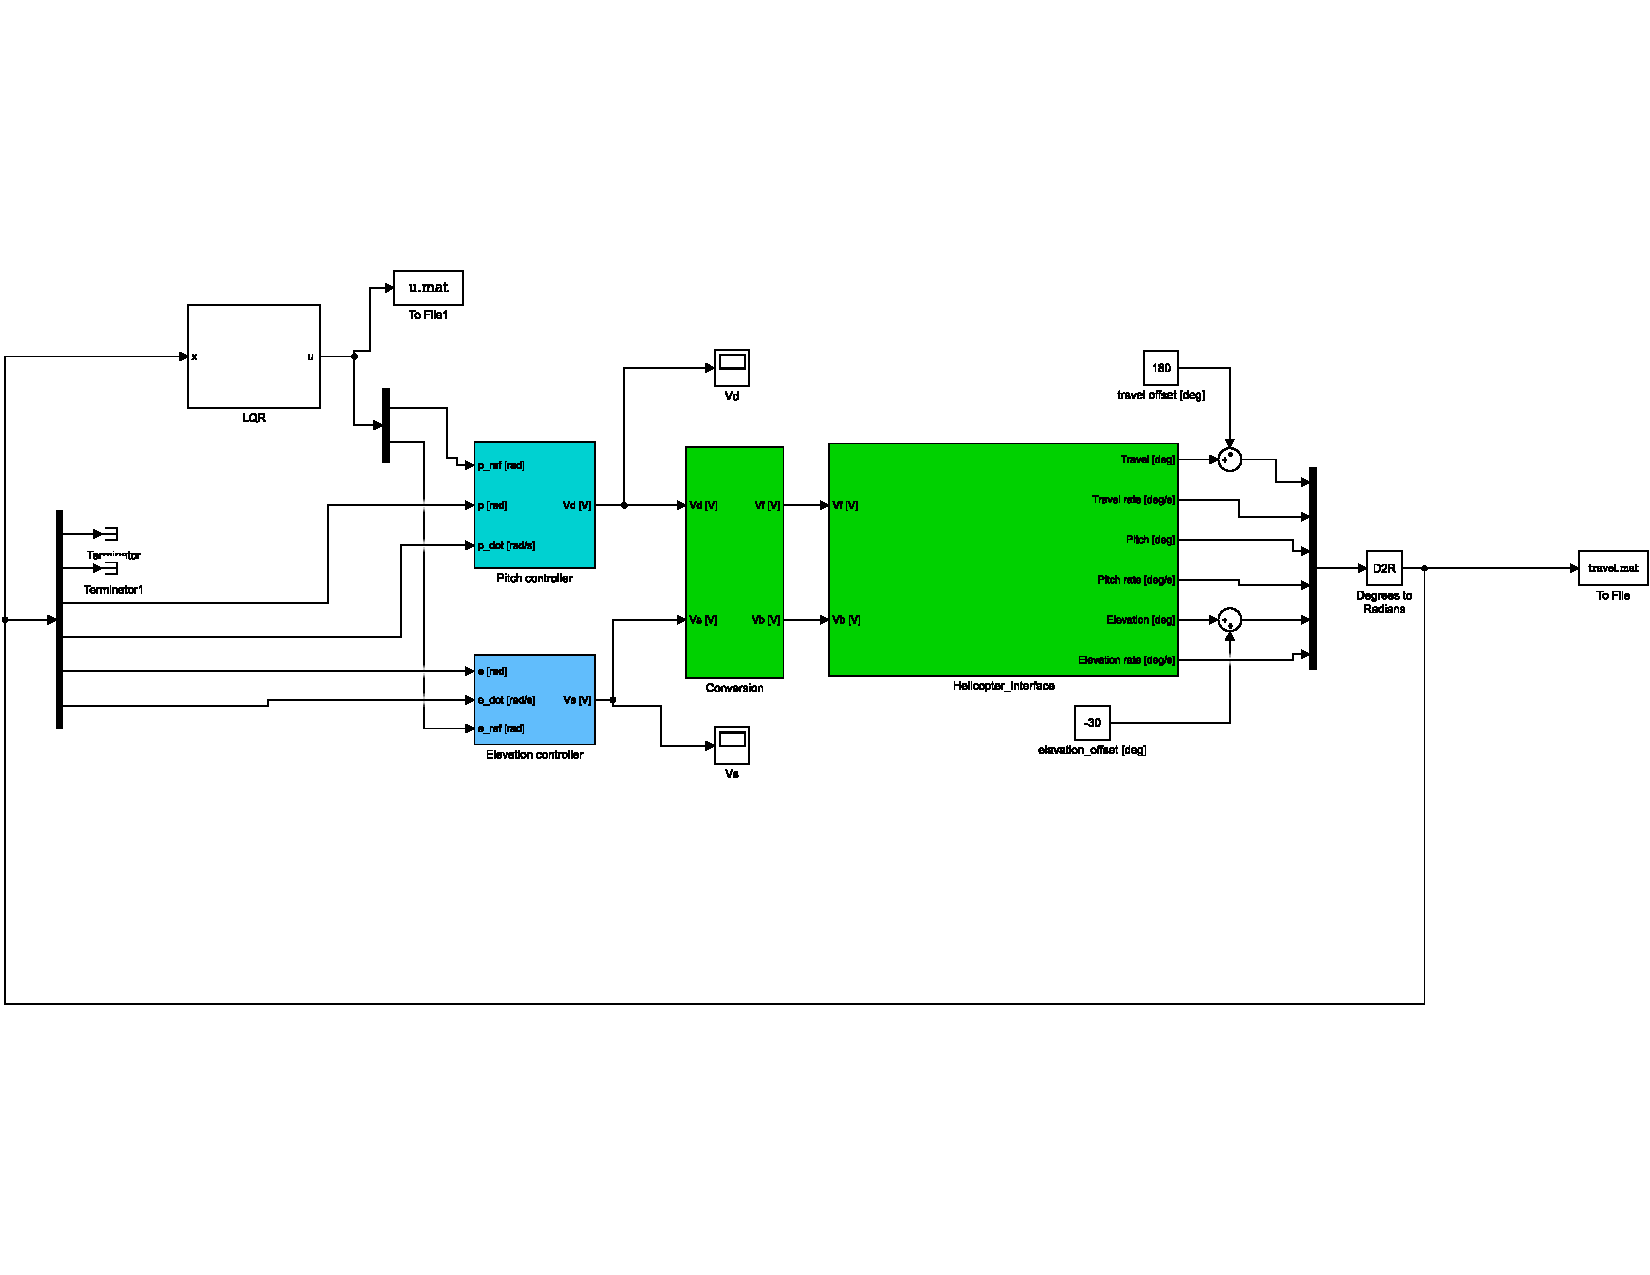
\includegraphics[scale=0.5]{data_10.4/simulink.pdf}
    \caption{Simulink model for problem 10.4}
    \label{fig:10_4_simulink}
\end{figure}
\begin{figure}[H]
    \centering
    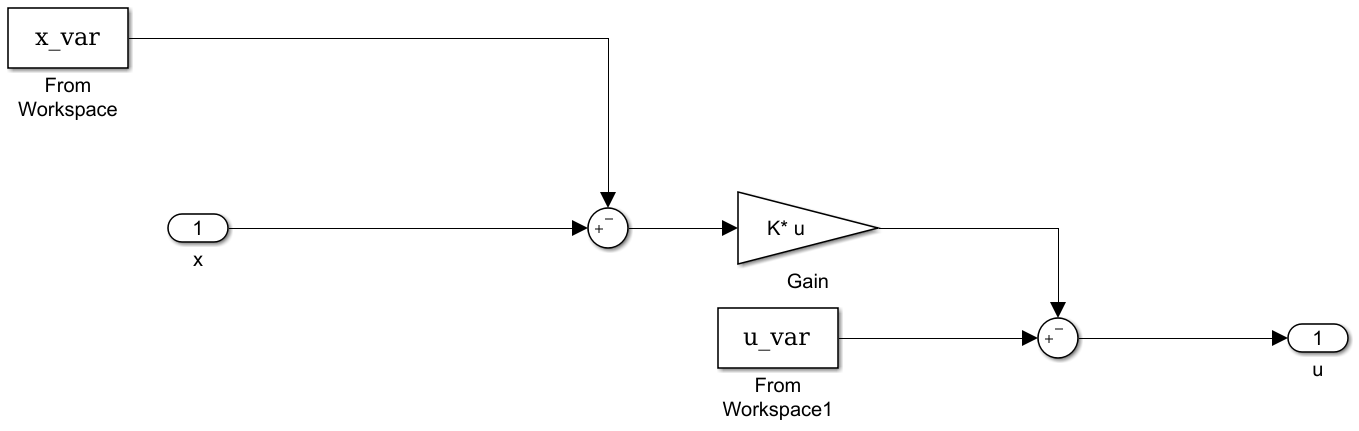
\includegraphics[width=1\linewidth]{data_10.4/simmodel_lqr.PNG}
    \caption{Simulink model showing the block diagram in LQR for problem 10.4}
    \label{fig:10_4_simulink_lqr}
\end{figure}


% References
\newpage
\addcontentsline{toc}{section}{References}
\printbibliography{}
\label{sec:bibliography}

\end{document}
